\newpage

\begin{table}[ht]
\centering
\caption{1B LLM English evaluation. Each trial requires approximately 11.3k A100-40G hours.}
\label{tab:lm_results_rebuttal}
\begin{sc}
\begin{scriptsize}
\bgroup
\setlength{\tabcolsep}{.35em}
\begin{tabular}{@{}lllllllllllllll@{}}
\toprule
Model   & \makecell{Seq.\\Len.} & \makecell{ARC\\Easy} & \makecell{ARC\\Challenge} & \makecell{Hella-\\swag} & Piqa & Sciq & \makecell{Wino-\\grande} & \makecell{Lambada\\OpenAI} & \makecell{TriviaQA\\(1-shot)} & \makecell{WebQS\\(1-shot)} & AVG & \makecell{Step\\time (s)} \\ \midrule
Softmax (ALiBi) & 2k & 62.2       &     26.8           &    42.4       &  59.0    &   72.3   &     88.1       &     58.4           &      19.9             &    15.4            &    49.4   & 0.38   \\
Sigmoid (ALiBi) & 2k &  62.8       &      28.8         &    42.5       &  59.7    &   70.3   &     88.6       &      59.7          &       19.1            &   13.8             &       49.5  & 0.34   \\
\midrule
Softmax (RoPE) & 4k & 63.3       &     29.3           &    43.3       &  58.1    &   71.3   &     86.9       &     58.8           &  20.4             &    15.6            &    49.7   & 0.84   \\
Softmax (ALiBi) & 4k & 62.6       &     27.7           &    42.4       &  58.6    &   71.1   &     88.2       &     58.6           &      18.9             &    14.7            &    49.2   & 0.84   \\
Sigmoid (ALiBi) & 4k &  60.5       &      27.3         &    41.3       &  57.8    &   70.5   &     87.0       &      57.6          &       18.9            &   12.6             &       48.2  & 0.67   \\ \bottomrule
\end{tabular}
\egroup
\end{scriptsize}
\end{sc}
\vspace{-0.4cm}
\end{table}
\begin{figure}[ht]
  \begin{minipage}{0.7\textwidth}
    \centering
    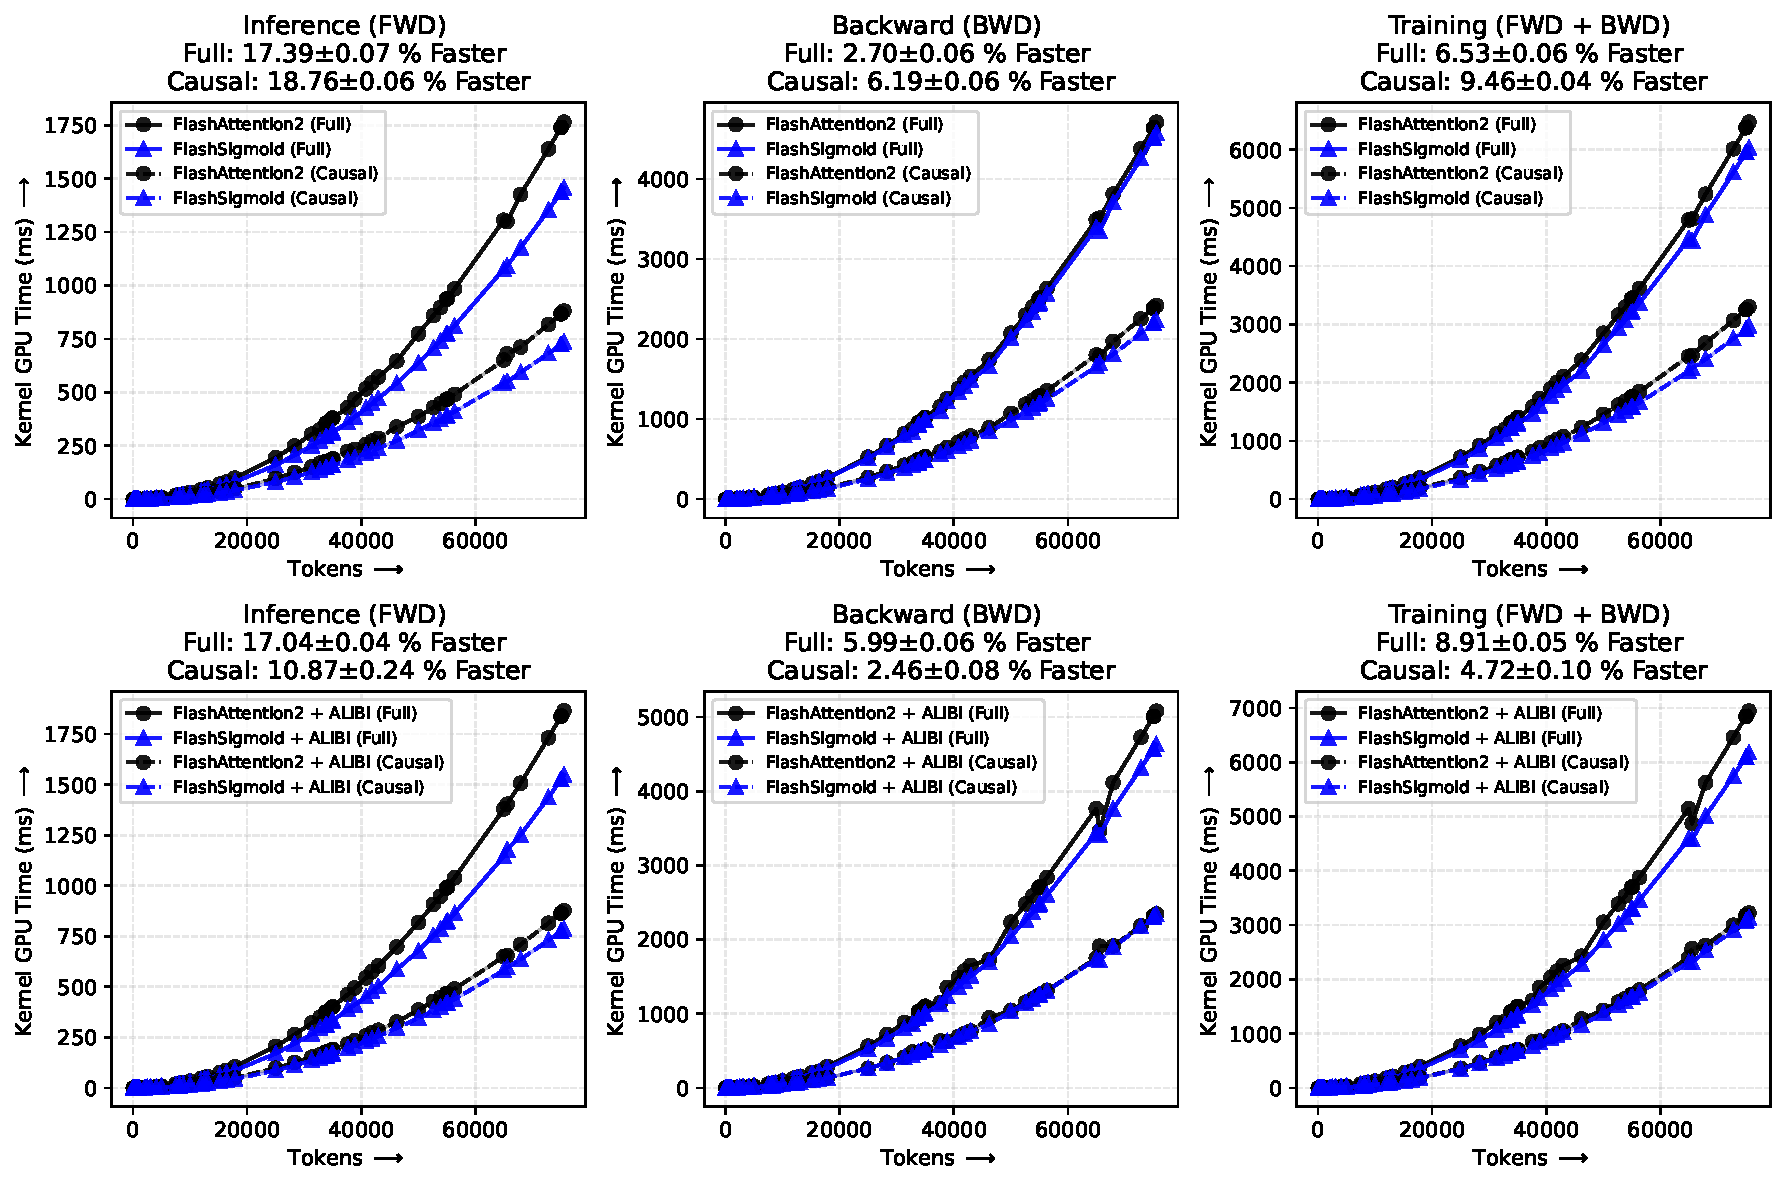
\includegraphics[width=\linewidth]{figures/_flash_figures/rebuttal/H100_all_major.pdf}
  \end{minipage}%
  \hfill
  \begin{minipage}{0.29\textwidth}
    \caption{Updated H100 kernel timings for FlashSigmoid.
    Top row compares FlashSigmoid vs. FlashAttention2 without ALiBi and the bottom row compares with ALiBi.
    Each subplot lists the average speedup over all tokens. 
    Benchmarking is performed on 8 different H100 GPUs to cater for internode variance. 
    In all cases FlashSigmoid is faster on average for all tokens. In real end-to-end tests we observe a 8.62\% speedup at sequence length 10,000.
    }
    \label{fig:h100_kernel_benchmarking_rebuttal}
  \end{minipage}  
\end{figure}
\vspace{-0.1in}
\subsection{Sigmoid Attention vs. Attention Relaxations}
\label{sec:attention_relaxations}
\vspace{-0.1in}
\begin{figure}[ht]
   \begin{minipage}{0.5\textwidth}
    \centering
    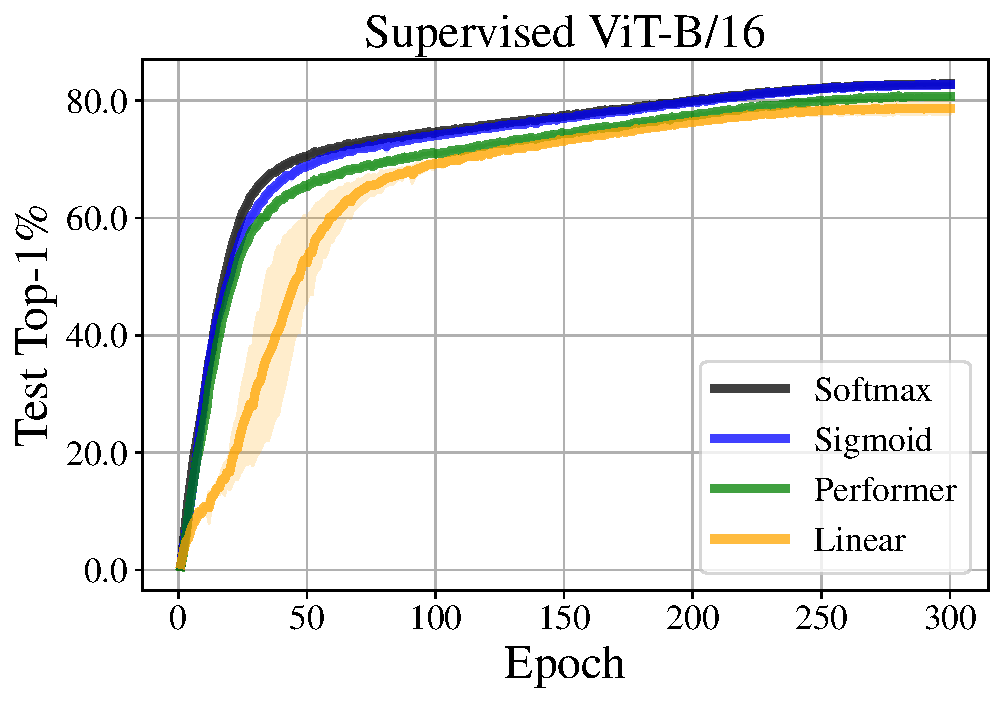
\includegraphics[width=\linewidth]{figures/test_top1_attn_relaxations.pdf}
  \end{minipage}%
  \hfill
  \begin{minipage}{0.48\textwidth}
    \caption{Supervised ViT-B/16 ImageNet1k classification. We contrast $\sigmoidattn$ and $\softmaxattn$ against (a) linear attention with no activation: $\mQ \mK^T / \sqrt{d_{qk}}$ and (b) fast attention via positive orthogonal random features, used in Performer \citep{DBLP:conf/iclr/ChoromanskiLDSG21}. $\sigmoidattn$, like $\softmaxattn$, differs from attention relaxations like Performer which uses low-rank representations of the attention matrix. $\sigmoidattn$ maintains performance parity with $\softmaxattn$, while outperforming other efficient attention variants.}
    \label{fig:attention_relaxations}
  \end{minipage}  
\end{figure}
\vspace{-0.1in}
\subsection{Computational Complexity of Sigmoid and Softmax.}
\label{sec:parameter_and_flops}
\vspace{-0.1in}
\begin{table}[h!]
\small
\centering
\caption{Forward floating operations per token per attention head. 
$n_\text{ctx}$ and $d_\text{head}$ are the context length and head dimension respectively. 
$\Delta$ measures the compute difference between sigmoid and softmax as a multiple of the floating operations for computing the attention logits. 
$c$ accounts for causal ($c=(n_\text{ctx}+1)/2n_\text{ctx}\sim1/2$), or standard ($c=1$) attention.
Typical values are taken from the 1B LLM results ($n_\text{ctx}=2048$, $d_\text{head}=64$).
The difference in floating operations between Sigmoid and Softmax attention mechanisms is subleading ($\sim1\%$) compared to other operations in the attention mechanism like computing attention logits $\mL$ (shown below), and the attention matrix $\times$ values operation. This analysis precludes hardware aware improvements (\Cref{sec:FlashSigmoidHardwareAwareImplementation}).
}
\label{tab:flop-counts}
\begin{tabular}{lcccc}
\toprule
& $\mL=\mQ\mK^T$ & $\softmax\left(\mL\right)$ & $\sigmoid\left(\mL+\vb\right)$ & $\Delta$ \\ \midrule 
Expression & $ 2\,c\,n_\text{ctx}\,d_{\text{head}}$ & $ 3\,c\,n_\text{ctx}$ & $ 5\,c\,n_\text{ctx}$ & $1/d_{\text{head}}$\\
Value & $262144\,c$ & $6144\,c$ & $10240\,c$ & $1/64$ \\ \bottomrule
\end{tabular}
\end{table}



